\section{Specifica componenti Romeo::Controller}
\subsection{Romeo::Controller}
	\begin{figure} [!h]
		\centering
		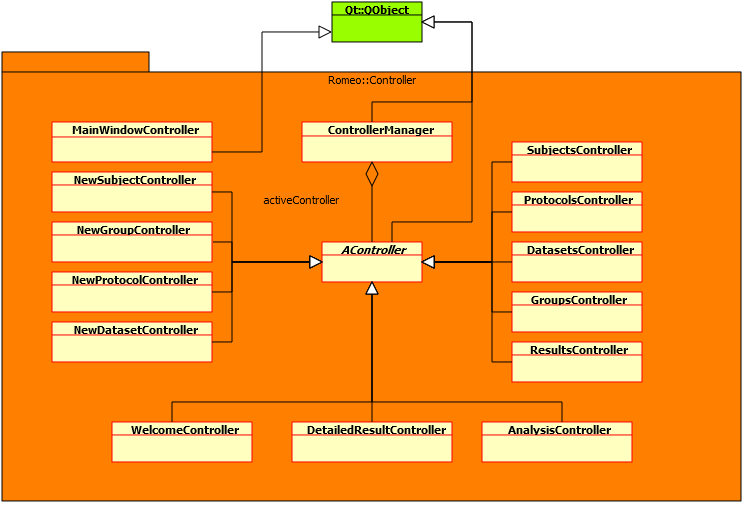
\includegraphics[scale=0.5] {../Specifica_Tecnica/Content/Immagini/Romeo__Controller.png}
		\caption{Diagramma package \textsl{Romeo::Controller}}
	\end{figure}
	\subsubsection{AController (abstract)}
	\begin{figure}[!h]
		\centering
		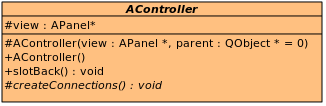
\includegraphics[width=0.5\linewidth]{./Content/Immagini/controller/AController.png}
		\caption{Diagramma classe \textsl{AController}}
	\end{figure}
	\paragraph{Descrizione:} classe astratta che rappresenta un generico controller per un oggetto derivato dalla classe \textsl{APanel}
	\paragraph{Utilizzo:} riceve i signal\g{} dalla vista che sta gestendo e reagisce di conseguenza.
	\paragraph{Eredita da:}
		\begin{itemize}
			\item Qt::QObject.
		\end{itemize}
	\paragraph{Attributi}
		\begin{itemize}
			\item \color{teal} \verb!# view : APanel *!
			\color{black}
			\subparagraph{Descrizione} Puntatore all'oggetto \textsl{APanel} che l'oggetto \textsl{AController} sta controllando. Essendo \textsl{APanel} una classe astratta, il tipo dinamico di tale puntatore non sarà mai \verb!APanel *!, ma bensì un puntatore ad una sua sottoclasse.
		\end{itemize}
	\paragraph{\color{black}Metodi}
		\begin{itemize}
			\item \color{blue} \verb!# AController(view : APanel *, parent : QObject *)!
			\color{black}
			\subparagraph{Descrizione:} Costruttore protetto che crea un controller sull'oggetto view passato come parametro.
			\color{black}
			\subparagraph{Argomenti}
			\begin{itemize}
				\item \color{RoyalPurple} \verb!view : APanel *!\\				
\color{black} Puntatore all'oggetto \textsl{APanel} al quale lavorerà l'oggetto \textsl{AController} che verrà costruito.
				\item \color{RoyalPurple} \verb!parent : QObject *!\\				
\color{black} Puntatore all'oggetto \textsl{QObject} padre dell'oggetto \textsl{AController}.
			\end{itemize}
			\item \color{blue} \verb!# createConnections() : void!
			\color{black}
			\subparagraph{Descrizione} Metodo virtuale puro che fornisce un contratto per la creazione delle varie connect per gestire i signal\g{} inviati dalla view.
			\subparagraph{Note}
			\begin{itemize}
				\item Il metodo deve essere marcato come costante.
				\item Il metodo deve essere marcato come virtuale puro.
			\end{itemize}
			\item \color{blue} \verb!+ slotBack() : void!
			\color{black}
			\subparagraph{Descrizione} Metodo che gestisce la richiesta, da parte dell'utente, di ritornare alla vista precedente.
			\subparagraph{Note}
			\begin{itemize}
				\item Il metodo deve essere marcato come virtuale.
			\end{itemize}
		\end{itemize}
	\pagebreak
	\subsubsection{AnalysisController (class)}
	\begin{figure}[!h]
		\centering
		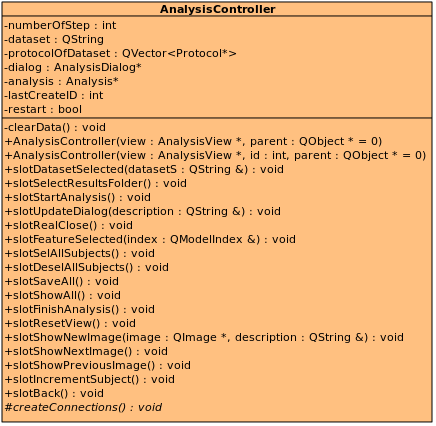
\includegraphics[width=0.65\linewidth]{./Content/Immagini/controller/AnalysisController.png}
		\caption{Diagramma classe AnalysisController}
	\end{figure}
	\paragraph{Descrizione:} classe che rappresenta il controller per un oggetto AnalysisView.
	\paragraph{Utilizzo:} viene utilizzata per gestire i Signal\g{} emessi da un oggetto Analysisview e reagisce in modo appropriato ogni volta che ne viene catturato uno.
	\paragraph{Eredita da:}
		\begin{itemize}
			\item Romeo::Controller::AController.
		\end{itemize}
	\paragraph{Attributi}
		\begin{itemize}
			\item \color{teal} \verb!- dataset : QString!
			\color{black}
			\subparagraph{Descrizione} contiene il nome del Dataset\g{} da analizzare
			\item \color{teal} \verb!- dialog : AnalysisDialog *!
			\color{black}
			\subparagraph{Descrizione} rappresenta il puntatore alla finestra di dialogo per iniziare l'analisi.
			\item \color{teal} \verb!- analysis : Analysis *!
			\color{black}
			\subparagraph{Descrizione} puntatore all'oggetto analysis
			\item \color{teal} \verb!- lastCreateID : int!
			\color{black}
			\subparagraph{Descrizione} rappresenta l'id nel database dell'analisi corrente creata.
			\item \color{teal} \verb!- restart : bool!
			\color{black}
			\subparagraph{Descrizione} rappresenta un flag che vale false se l'analisi è una nuova analisi true altrimenti.
			\item \color{teal} \verb!- protocolsOfDataset : QVector<Protocol*>!
			\color{black}
			\subparagraph{Descrizione} rappresenta i Protocol\g{} contenuti nel Dataset\g{} del quale si vuole fare l'analisi.
		\end{itemize}
	\paragraph{\color{black}Metodi}
		\begin{itemize}
			\item \color{blue} \verb!- clearData() : void!
			\color{black}
			\subparagraph{Descrizione} metodo che rimuove i dati dell'oggetto controllore
			\item \color{blue} \verb!- createDialogConnections() : void!
			\color{black}
			\subparagraph{Descrizione} metodo che crea le connessioni per la finestra di dialogo di inizio analisi.
			\item \color{blue} \verb!# createConnections() : void!
			\color{black}
			\subparagraph{Descrizione} metodo che ha il compito di creare le connessioni tra la vista che l'oggetto controllore ha associata e il controller stesso.
			\subparagraph{Note}
			\begin{itemize}
				\item Il metodo deve essere marcato come costante.
			\end{itemize}
			\item \color{blue} \verb!+ AnalysisController(analysis : Analysis *, parent : QObject *)!
			\color{black}
			\subparagraph{Descrizione:} costruttore per la creazione del controller di una nuova analisi
			\color{black}
			\subparagraph{Argomenti}
			\begin{itemize}
				\item \color{RoyalPurple} \verb!analysis : Analysis *!\\				
\color{black} puntatore alla view associata al controller.
				\item \color{RoyalPurple} \verb!parent : QObject *!\\				
\color{black} rappresenta il parent dell'oggetto controller in costruzione.
			\end{itemize}
			\item \color{blue} \verb!+ AnalysisController(analysis : Analysis *, id : int, parent : QObject *)!
			\color{black}
			\subparagraph{Descrizione:} costruttore per la classe che ha il compito di creare il controller per un'analisi già esistente da far ripartire.
			\color{black}
			\subparagraph{Argomenti}
			\begin{itemize}
				\item \color{RoyalPurple} \verb!analysis : Analysis *!\\				
\color{black} puntatore alla vista associata al controller in costruzione.
				\item \color{RoyalPurple} \verb!id : int!\\				
\color{black} rappresenta l'id univoco dell'oggetto analisi all'interno del database.
				\item \color{RoyalPurple} \verb!parent : QObject *!\\				
\color{black} rappresenta il parent dell'oggetto in costruzione
			\end{itemize}
			\item \color{blue} \verb!+ slotDatasetSelected(datasetS : const QString &) : void!
			\color{black}
			\subparagraph{Descrizione:} Slot\g{} che riceve il segnale dalla view associata quando l'utente seleziona un dataset.
			\color{black}
			\subparagraph{Argomenti}
			\begin{itemize}
				\item \color{RoyalPurple} \verb!datasetS : const QString &!\\				
\color{black} rappresenta il nome del Dataset\g{} selezionato.
			\end{itemize}
			\subparagraph{Note}
			\begin{itemize}
				\item Il metodo è uno slot\g{} Qt\g{}.
			\end{itemize}
			\item \color{blue} \verb!+ slotSelectedResultsFolder() : void!
			\color{black}
			\subparagraph{Descrizione} Slot\g{} che riceve il segnale dalla view associata quando l'utente seleziona il pulsante per la cartella in cui verranno esportati i risultati che l'analisi produrrà.
			\subparagraph{Note}
			\begin{itemize}
				\item Il metodo è uno slot\g{} Qt\g{}.
			\end{itemize}
			\item \color{blue} \verb!+ slotStartAnalysis() : void!
			\color{black}
			\subparagraph{Descrizione} Slot\g{} che riceve il segnale dalla view associata quando l'utente seleziona il pulsante per iniziare l'analisi.
			\subparagraph{Note}
			\begin{itemize}
				\item Il metodo è uno slot\g{} Qt\g{}.
			\end{itemize}
			\item \color{blue} \verb!+ slotUpdateDialog(description : const QString &) : void!
			\color{black}
			\subparagraph{Descrizione:} Slot\g{} che riceve il segnale dalla view associata quando la finestra di dialogo dell'analisi necessita di aggiornare la vista.
			\color{black}
			\subparagraph{Argomenti}
			\begin{itemize}
				\item \color{RoyalPurple} \verb!description : const QString &!\\				
\color{black} rappresenta la descrizione testuale da impostare alla view.
			\end{itemize}
			\subparagraph{Note}
			\begin{itemize}
				\item Il metodo è uno slot\g{} Qt\g{}.
			\end{itemize}
			\item \color{blue} \verb!+ slotRealClose() : void!
			\color{black}
			\subparagraph{Descrizione} Slot\g{} che riceve il segnale dalla view associata quando la finestra di dialogo ha terminato l'analisi e imposta i puntatori analysis e dialog a null.
			\subparagraph{Note}
			\begin{itemize}
				\item Il metodo è uno slot\g{} Qt\g{}.
			\end{itemize}
			\item \color{blue} \verb!+ slotFeatureSelected(index : const QModelIndex &) : void!
			\color{black}
			\subparagraph{Descrizione:} Slot\g{} che riceve il segnale dalla view associata quando l'utente seleziona le Feature\g{} da visualizzare o salvare.
			\color{black}
			\subparagraph{Argomenti}
			\begin{itemize}
				\item \color{RoyalPurple} \verb!index : const QModelIndex &!\\				
\color{black} rappresenta l'indice della tabella selezionata dall'utente.
			\end{itemize}
			\subparagraph{Note}
			\begin{itemize}
				\item Il metodo è uno slot\g{} Qt\g{}.
			\end{itemize}
			\item \color{blue} \verb!+ slotSelAllSubjects() : void!
			\color{black}
			\subparagraph{Descrizione} Slot\g{} che riceve il segnale dalla view associata quando l'utente preme il pulsante per selezionare tutti i Subject\g{} presenti nel Dataset\g{}.
			\subparagraph{Note}
			\begin{itemize}
				\item Il metodo è uno slot\g{} Qt\g{}.
			\end{itemize}
			\item \color{blue} \verb!+ slotDeselAllSubject() : void!
			\color{black}
			\subparagraph{Descrizione} Slot\g{} che riceve il segnale dalla view associata quando l'utente preme il pulsante per deselezionare tutti i Subject\g{} presenti nel Dataset\g{}.
			\subparagraph{Note}
			\begin{itemize}
				\item Il metodo è uno slot\g{} Qt\g{}.
			\end{itemize}
			\item \color{blue} \verb!+ slotSaveAll() : void!
			\color{black}
			\subparagraph{Descrizione} Slot\g{} che riceve il segnale dalla view associata quando l'utente preme il pulsante per salvare tutte le Feature\g{} presenti.
			\subparagraph{Note}
			\begin{itemize}
				\item Il metodo è uno slot\g{} Qt\g{}.
			\end{itemize}
			\item \color{blue} \verb!+ slotShowAll() : void!
			\color{black}
			\subparagraph{Descrizione} Slot\g{} che riceve il segnale dalla view associata quando l'utente preme il pulsante per visualizzare tutte le Feature\g{} presenti.
			\subparagraph{Note}
			\begin{itemize}
				\item Il metodo è uno slot\g{} Qt\g{}.
			\end{itemize}
			\item \color{blue} \verb!+ slotFinishAnalysis() : void!
			\color{black}
			\subparagraph{Descrizione} Slot\g{} che riceve il segnale dalla view associata quando l'analisi è stata terminata.
			\subparagraph{Note}
			\begin{itemize}
				\item Il metodo è uno slot\g{} Qt\g{}.
			\end{itemize}
			\item \color{blue} \verb!+ slotResetView() : void!
			\color{black}
			\subparagraph{Descrizione} Slot\g{} che riceve il segnale dalla view associata per ripristinare la view.
			\subparagraph{Note}
			\begin{itemize}
				\item Il metodo è uno slot\g{} Qt\g{}.
			\end{itemize}
			\item \color{blue} \verb!+ slotShowNewImage(image : QImage *, description : const QString &) : void!
			\color{black}
			\subparagraph{Descrizione:} Slot\g{} che riceve il segnale dalla view associata quando la nuova immagine dell'analisi è pronta per essere mostrata.
			\color{black}
			\subparagraph{Argomenti}
			\begin{itemize}
				\item \color{RoyalPurple} \verb!image : QImage *!\\				
\color{black} rappresenta l'immagine da mostrare.
				\item \color{RoyalPurple} \verb!description : const QString &!\\				
\color{black} rappresenta la descrizione dell'immagine  passata come parametro.
			\end{itemize}
			\subparagraph{Note}
			\begin{itemize}
				\item Il metodo è uno slot\g{} Qt\g{}.
			\end{itemize}
			\item \color{blue} \verb!+ slotShowNextImage() : void!
			\color{black}
			\subparagraph{Descrizione} Slot\g{} che riceve il segnale dalla view associata quando l'utente preme il pulsante per visualizzare l'immagine successiva dalla finestra di dialogo.
			\subparagraph{Note}
			\begin{itemize}
				\item Il metodo è uno slot\g{} Qt\g{}.
			\end{itemize}
			\item \color{blue} \verb!+ slotShowPreviousImage() : void!
			\color{black}
			\subparagraph{Descrizione} Slot\g{} che riceve il segnale dalla view associata quando l'utente preme il pulsante per visualizzare l'immagine precedente dalla finestra di dialogo.
			\subparagraph{Note}
			\begin{itemize}
				\item Il metodo è uno slot\g{} Qt\g{}.
			\end{itemize}
			\item \color{blue} \verb!+ slotIncrementSubject() : void!
			\color{black}
			\subparagraph{Descrizione} Slot\g{} che riceve il segnale dalla view associata per aumentare il numero di Subject\g{}da analizzare.
			\subparagraph{Note}
			\begin{itemize}
				\item Il metodo è uno slot\g{} Qt\g{}.
			\end{itemize}
			\item \color{blue} \verb!+ slotBack() : void!
			\color{black}
			\subparagraph{Descrizione} Slot\g{} che riceve il segnale dalla view associata quando l'utente preme il pulsante back per tornare alla view precedente.
			\subparagraph{Note}
			\begin{itemize}
				\item Il metodo deve essere marcato come virtuale.
				\item Il metodo è uno slot\g{} Qt\g{}.
			\end{itemize}
		\end{itemize}
		\pagebreak
	\subsubsection{ControllerManager (class)}
	\begin{figure}[!h]
		\centering
		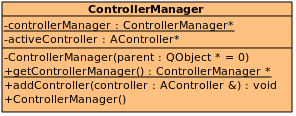
\includegraphics[width=0.6\linewidth]{./Content/Immagini/controller/ControllerManager}
		\caption{Diagramma classe \textsl{ControllerManager}}
	\end{figure}
	\paragraph{Descrizione:} classe che si occupa di cancellare i controller dalla memoria, quando non sono più necessari. È implementata tramite il design patterng\g{} Singleton.
	\paragraph{Utilizzo:} si occupa di gestire ed eliminare i controller.
	\paragraph{Eredita da:}
		\begin{itemize}
			\item Qt::QObject.
		\end{itemize}
	\paragraph{Attributi}
		\begin{itemize}
			\item \color{teal} \verb!- activeController : AController *!
			\color{black}
			\subparagraph{Descrizione} Puntatore al controller attivo in un determinato istante.
			\item \color{teal} \verb!- static controllerManager : ControllerManager *!
			\color{black}
			\subparagraph{Descrizione} Puntatore al campo dati statico che rappresenta l'unica istanza della classe ControllerManager. Tale istanza verrà creata in modo \textit{lazy}, ossia non sarà creata prima di quando viene richiesta per la prima volta.
		\end{itemize}
	\paragraph{\color{black}Metodi}
		\begin{itemize}
			\item \color{blue} \verb!- ControllerManager(parent : QObject *)!
			\color{black}
			\subparagraph{Descrizione:} Costruttore privato, come previsto dal design patterng\g{} Singleton, della classe \textsl{ControllerManger}. Essendo privato, non sarà possibile creare direttamente oggetti di tipo \textsl{ControllerManager}. Per ottenere l'unica istanza di \textsl{ControllerManger} si dovrà utilizzare il metodo \verb!getControllerManager()!.
			\color{black}
			\subparagraph{Argomenti}
			\begin{itemize}
				\item \color{RoyalPurple} \verb!parent : QObject *!\\				
\color{black} Puntatore al \textsl{QObject} padre dell'oggetto \textsl{ControllerManger}.
			\end{itemize}
			\item \color{blue} \verb!+ getControllerManger() : ControllerManager *!
			\color{black}
			\subparagraph{Descrizione} Metodo statico che, come previsto dal design patterng\g{} Singleton, ritorna l'unica istanza della classe \textsl{ControllerManager} esistente. Se tale istanza non è ancora esitente, il metodo si occuperà di crearla.
			\item \color{blue} \verb!+ addController(controller : const AController &) : void!
			\color{black}
			\subparagraph{Descrizione:} Metodo che permette di impostare l'oggetto di tipo \textsl{AController} attivo in un dato instante. Se al momento della chiamata è già presente un oggetto \textsl{AController}, esso viene eliminato dalla memoria. In questo modo non si ha memoria inutilizzata.
			\color{black}
			\subparagraph{Argomenti}
			\begin{itemize}
				\item \color{RoyalPurple} \verb!controller : const AController &!\\				
\color{black} Rappresenta l'oggetto \textsl{AController} da gestire.
			\end{itemize}
		\end{itemize}
		\pagebreak
	\subsubsection{DatasetsController (class)}
	\begin{figure}[!h]
		\centering
		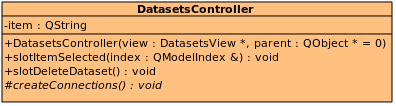
\includegraphics[width=0.6\linewidth]{./Content/Immagini/controller/DatasetsController}
		\caption{Diagramma classe \textsl{DatasetsController}}
	\end{figure}
	\paragraph{Descrizione:} classe rappresentante un controller per un oggetto di tipo \textsl{DatasetsView}.
	\paragraph{Utilizzo:} gestisce i signal\g{} emessi da un oggetto \textsl{DatasetsView} ed agisce conseguentemente in modo appropriato.
	\paragraph{Eredita da:}
		\begin{itemize}
			\item Romeo::Controller::AController.
		\end{itemize}
	\paragraph{Attributi}
		\begin{itemize}
			\item \color{teal} \verb!- item : QString!
			\color{black}
			\subparagraph{Descrizione} Rappresenta il nome del Dataset\g{} selezionato dall'utente nella vista associata al controller.
		\end{itemize}
	\paragraph{\color{black}Metodi}
		\begin{itemize}
			\item \color{blue} \verb!# createConnections() : void!
			\color{black}
			\subparagraph{Descrizione} Metodo che si occupa di creare le connessioni tra i segnali emessi dalla vista associata e gli slot\g{} dell'oggetto \textsl{DatasetsController}.
			\subparagraph{Note}
			\begin{itemize}
				\item Il metodo deve essere marcato come costante.
				\item Il metodo deve essere marcato come virtuale.
			\end{itemize}
			\item \color{blue} \verb!+ DatasetsController(view : DatasetsView *, parent : QObject *)!
			\color{black}
			\subparagraph{Descrizione:} Costruttore protetto della classe \textsl{DatasetsController}. Si occupa di costruire un oggetto di tipo \textsl{DatasetsController}, associandolo alla propria vista.
			\color{black}
			\subparagraph{Argomenti}
			\begin{itemize}
				\item \color{RoyalPurple} \verb!view : DatasetsView *!\\				
\color{black} Puntatore all'oggetto di tipo \textsl{DatasetView}, rappresentante la vista che verrà controllata dall'oggetto \textsl{DatasetsController}.
				\item \color{RoyalPurple} \verb!parent : QObject *!\\				
\color{black} Puntatore all'oggetto \textsl{QObject}, rappresentante il padre dell'oggetto \textsl{DatasetsController}.
			\end{itemize}
			\item \color{blue} \verb!+ slotItemSelected(index : const QModelIndex &) : void!
			\color{black}
			\subparagraph{Descrizione:} Metodo pubblico che mostra i dettagli del Dataset\g{} selezionato dall'utente, nella vista associata.
			\color{black}
			\subparagraph{Argomenti}
			\begin{itemize}
				\item \color{RoyalPurple} \verb!index : const QModelIndex &!\\				
\color{black} Indice dell'item associato al Dataset\g{} selezionato dall'utente.
			\end{itemize}
			\subparagraph{Note}
			\begin{itemize}
				\item Il metodo è uno slot\g{} Qt\g{}.
			\end{itemize}
			\item \color{blue} \verb!+ slotDeleteDataset() : void!
			\color{black}
			\subparagraph{Descrizione} Elimina il Dataset\g{} selezionato dall'utente dal database.
			\subparagraph{Note}
			\begin{itemize}
				\item Il metodo è uno slot\g{} Qt\g{}.
			\end{itemize}
			\item \color{blue} \verb!- featuresInfo(feats : QVector<AFeature*>, txtProtocols : QString &) : void!
			\color{black}
			\subparagraph{Descrizione:} aggiunge le informazioni riguardanti le Feature\g{} alla stringa passata come parametro.
			\color{black}
			\subparagraph{Argomenti}
			\begin{itemize}
				\item \color{RoyalPurple} \verb!feats : QVector<AFeature*>!\\				
\color{black} rappresenta puntatori alle Feature\g{} presenti nei Protocol\g{} del Datase\g{} preso in considerazione.
				\item \color{RoyalPurple} \verb!txtProtocols : QString &!\\				
\color{black} rappresenta la stringa al quale vengono aggiunte le informazioni relative alle Feature\g{}.
			\end{itemize}
			\subparagraph{Note}
			\begin{itemize}
				\item Il metodo deve essere marcato come costante.
			\end{itemize}
			\item \color{blue} \verb!- algorithmInfo(alg : AAlgorithm *, txtProtocols : QString &) : void!
			\color{black}
			\subparagraph{Descrizione:} aggiunge le informazioni riguardanti l'algoritmo di cluster\g{} alla stringa passata come parametro.
			\color{black}
			\subparagraph{Argomenti}
			\begin{itemize}
				\item \color{RoyalPurple} \verb!alg : AAlgorithm *!\\				
\color{black} puntatore all'algoritmo contenuto nel Dataset\g{} selezionato.
				\item \color{RoyalPurple} \verb!txtProtocols : QString &!\\				
\color{black} stringa dove verranno aggiunte le informazioni riguardanti l'algoritmo.
			\end{itemize}
			\subparagraph{Note}
			\begin{itemize}
				\item Il metodo deve essere marcato come costante.
			\end{itemize}
		\end{itemize}
		\pagebreak
	\subsubsection{DetailedResultController (class)}
	\begin{figure}[!h]
		\centering
		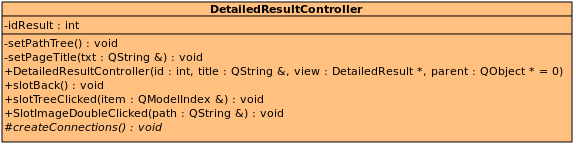
\includegraphics[width=0.75\linewidth]{./Content/Immagini/controller/DetailedResultController.png}
		\caption{Diagramma classe DetailedResultController}
	\end{figure}
	\paragraph{Descrizione:} La classe estende la classe astratta \textsl{AController} e ha il compito di catturare gli input dell'utente nella vista dei dettaglio risultati
	\paragraph{Utilizzo:} viene utilizzata per gestire i Signal\g{} emessi da un oggetto DetailedResultView e reagisce in modo appropriato
	\paragraph{Eredita da:}
		\begin{itemize}
			\item Romeo::Controller::AController.
		\end{itemize}
	\paragraph{Attributi}
		\begin{itemize}
			\item \color{teal} \verb!- idResult : int!
			\color{black}
			\subparagraph{Descrizione} rappresenta l'id dell'analisi con cui è identificata all'interno del database.
		\end{itemize}
	\paragraph{\color{black}Metodi}
		\begin{itemize}
			\item \color{blue} \verb!- setPathTree() : void!
			\color{black}
			\subparagraph{Descrizione} metodo che ha il compito di impostare  il path della vista ad albero.
			\item \color{blue} \verb!- setPageTitle(txt : const QString &) : void!
			\color{black}
			\subparagraph{Descrizione:} metodo che imposta il titolo della pagina nella parte alta della finestra.
			\color{black}
			\subparagraph{Argomenti}
			\begin{itemize}
				\item \color{RoyalPurple} \verb!txt : const QString &!\\				
\color{black} rappresenta il testo da mettere come titolo.
			\end{itemize}
			\subparagraph{Note}
			\begin{itemize}
				\item Il metodo deve essere marcato come costante.
			\end{itemize}
			\item \color{blue} \verb!# createConnections() : void!
			\color{black}
			\subparagraph{Descrizione} metodo che ha il compito di impostare le connessioni dell'oggetto.
			\subparagraph{Note}
			\begin{itemize}
				\item Il metodo deve essere marcato come costante.
				\item Il metodo deve essere marcato come virtuale.
			\end{itemize}
			\item \color{blue} \verb!+ DetailedResultController(id : int, title : const QString &, !\\ \verb!view : DetailedResult*, parent : QObject *)!
			\color{black}
			\subparagraph{Descrizione:} Costruttore della classe, che ha il compito di creare l'oggetto e le connessioni alla view associata.
			\color{black}
			\subparagraph{Argomenti}
			\begin{itemize}
				\item \color{RoyalPurple} \verb!id : int!\\				
\color{black} rappresenta l'id associato all'analisi di cui si stanno visualizzando i risultati.
				\item \color{RoyalPurple} \verb!title : const QString &!\\				
\color{black} rappresenta il titolo da mettere alla pagina.
				\item \color{RoyalPurple} \verb!view : DetailedResult*!\\				
\color{black} rappresenta la view a cui il controller in costruzione verrà associata.
				\item \color{RoyalPurple} \verb!parent : QObject *!\\				
\color{black} rappresenta il parent dell'oggetto in creazione.
			\end{itemize}
			\item \color{blue} \verb!+ slotBack() : void!
			\color{black}
			\subparagraph{Descrizione} Slot\g{} che riceve il segnale della view associata quando l'utente preme il pulsante per tornare indietro.
			\subparagraph{Note}
			\begin{itemize}
				\item Il metodo è uno slot\g{} Qt\g{}.
			\end{itemize}
			\item \color{blue} \verb!+ slotTreeClicked(item : const QModelIndex &) : void!
			\color{black}
			\subparagraph{Descrizione:} Slot\g{} che riceve il segnale dalla view associata quanto l'utente preme sull'albero.
			\color{black}
			\subparagraph{Argomenti}
			\begin{itemize}
				\item \color{RoyalPurple} \verb!item : const QModelIndex &!\\				
\color{black} rappresenta l'elemento selezionato dall'albero.
			\end{itemize}
			\subparagraph{Note}
			\begin{itemize}
				\item Il metodo è uno slot\g{} Qt\g{}.
			\end{itemize}
			\item \color{blue} \verb!+ slotImageDoubleClicked(path : const QString &) : void!
			\color{black}
			\subparagraph{Descrizione:} Slot\g{} che riceve il segnale dalla view associata quando l'utente fa il doppio click sull'immagine/video.
			\color{black}
			\subparagraph{Argomenti}
			\begin{itemize}
				\item \color{RoyalPurple} \verb!path : const QString &!\\				
\color{black} rappresenta il path del file selezionato.
			\end{itemize}
			\subparagraph{Note}
			\begin{itemize}
				\item Il metodo è uno slot\g{} Qt\g{}.
			\end{itemize}
		\end{itemize}
		\pagebreak
	\subsubsection{GroupsController (class)}
	\begin{figure}[!h]
		\centering
		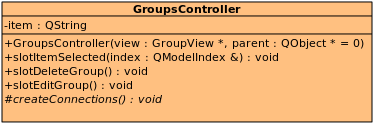
\includegraphics[width=0.6\linewidth]{./Content/Immagini/controller/GroupsController}
		\caption{Diagramma classe \textsl{GroupsController}}
	\end{figure}
	\paragraph{Descrizione:} classe che rappresenta un controller per un oggetto di tipo \textsl{GroupsView}.
	\paragraph{Utilizzo:} gestisce i signal\g{} emessi da un oggetto \textsl{GroupsView} ed agisce conseguentemente in modo appropriato.
	\paragraph{Eredita da:}
		\begin{itemize}
			\item Romeo::Controller::AController.
		\end{itemize}
	\paragraph{Attributi}
		\begin{itemize}
			\item \color{teal} \verb!- item : QString!
			\color{black}
			\subparagraph{Descrizione} Rappresenta il nome del gruppo di Subject\g{} selezionato dall'utente nella vista associata al controller.
		\end{itemize}
	\paragraph{\color{black}Metodi}
		\begin{itemize}
			\item \color{blue} \verb!# createConnections() : void!
			\color{black}
			\subparagraph{Descrizione} Metodo che si occupa di creare le connessioni tra i segnali emessi dalla vista associata e gli slot\g{} dell'oggetto \textsl{GroupsController}.
			\subparagraph{Note}
			\begin{itemize}
				\item Il metodo deve essere marcato come costante.
				\item Il metodo deve essere marcato come virtuale.
			\end{itemize}
			\item \color{blue} \verb!+ GroupsController(view : GroupView *, parent : QObject *)!
			\color{black}
			\subparagraph{Descrizione:} Costruttore pubblico della classe \textsl{GroupsController}. Si occupa di costruire un oggetto di tipo \textsl{GroupsController}, associandolo alla propria vista.
			\color{black}
			\subparagraph{Argomenti}
			\begin{itemize}
				\item \color{RoyalPurple} \verb!view : GroupView *!\\				
\color{black} Puntatore all'oggetto di tipo \textsl{GroupView}, rappresentante la vista che verrà controllata dall'oggetto \textsl{GroupsController}.
				\item \color{RoyalPurple} \verb!parent : QObject *!\\				
\color{black} Puntatore all'oggetto \textsl{QObject}, rappresentante il padre dell'oggetto \textsl{GroupsController}.
			\end{itemize}
			\item \color{blue} \verb!+ slotItemSelected(index : const QModelIndex &) : void!
			\color{black}
			\subparagraph{Descrizione:} Metodo pubblico che mostra i dettagli del gruppo di Subject\g{} selezionato dall'utente, nella vista associata.
			\color{black}
			\subparagraph{Argomenti}
			\begin{itemize}
				\item \color{RoyalPurple} \verb!index : const QModelIndex &!\\				
\color{black} Indice dell'item associato al gruppo di Subject\g{} selezionato dall'utente.
			\end{itemize}
			\subparagraph{Note}
			\begin{itemize}
				\item Il metodo è uno slot\g{} Qt\g{}.
			\end{itemize}
			\item \color{blue} \verb!+ slotDeleteGroup() : void!
			\color{black}
			\subparagraph{Descrizione} Elimina il gruppo di Subject\g{} selezionato dall'utente dal database.
			\subparagraph{Note}
			\begin{itemize}
				\item Il metodo è uno slot\g{} Qt\g{}.
			\end{itemize}
			\item \color{blue} \verb!+ slotEditGroup() : void!
			\color{black}
			\subparagraph{Descrizione} Metodo che permette all'utente di poter modificare il gruppo di Subject\g{} selezionato. Il metodo reindirizza l'utente ad un altra vista in cui può effettuare le dovute modifiche.
			\subparagraph{Note}
			\begin{itemize}
				\item Il metodo è uno slot\g{} Qt\g{}.
			\end{itemize}
		\end{itemize}
		\pagebreak
	\subsubsection{MainWindowController (class)}
	\begin{figure}[!h]
		\centering
		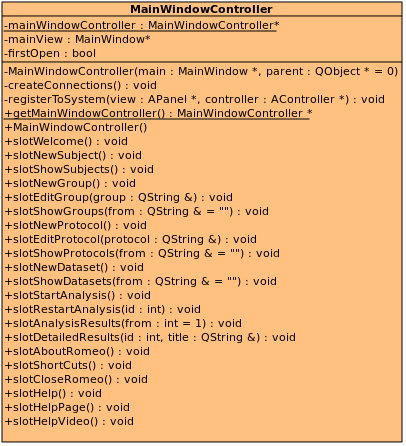
\includegraphics[width=0.75\linewidth]{./Content/Immagini/controller/MainViewController.png}
		\caption{Diagramma classe MainViewController}
	\end{figure}
	\paragraph{Descrizione:} classe che rappresenta un controller per un oggetto \textsl{MainWindowController}. Gestisce i vari input utente nella finestra principale del programma
	\paragraph{Utilizzo:} viene utilizzata per gestire i Signal\g{} emessi da un oggetto MainWindow. La classe MainWindowController recepisce i Signal\g{} emessi dalla view associata e reagisce in modo appropriato
	\paragraph{Eredita da:}
		\begin{itemize}
			\item Qt::QObject.
		\end{itemize}
	\paragraph{Attributi}
		\begin{itemize}
			\item \color{teal} \verb!- mainView : MainWindow*!
			\color{black}
			\subparagraph{Descrizione} rappresenta la main Window gestita dal mainWindowController.
			\item \color{teal} \verb!- firtOpen : bool!
			\color{black}
			\subparagraph{Descrizione} indica se la mainWindow è visualizzata per la prima volta (true).
			\item \color{teal} \verb!- static mainWindowController : MainWindowController*!
			\color{black}
			\subparagraph{Descrizione} rappresenta l'unica istanza di mainWindowController disponibile in quanto è stata implementando rispettando il design pattern\g{} Singleton.
			\subparagraph{Note}
			\begin{itemize}
				\item Il metodo deve essere marcato come static
			\end{itemize}
		\end{itemize}
	\paragraph{\color{black}Metodi}
		\begin{itemize}
			\item \color{blue} \verb!- MainWindowController(main : MainWindow*, parent : QObject *)!
			\color{black}
			\subparagraph{Descrizione:} costruttore per l'oggetto della classe MainWindowController in cui gli verrà associata la view passata come parametro.
			\color{black}
			\subparagraph{Argomenti}
			\begin{itemize}
				\item \color{RoyalPurple} \verb!main : MainWindow*!\\				
\color{black} rappresenta la view che verrà gestita dal controller in creazione.
				\item \color{RoyalPurple} \verb!parent : QObject *!\\				
\color{black} rappresenta il parent dell'oggetto in creazione.
			\end{itemize}
			\item \color{blue} \verb!- createConnections() : void!
			\color{black}
			\subparagraph{Descrizione} metodo che ha il compito di creare tutte le connessioni per l'oggetto della classe in questione.
			\subparagraph{Note}
			\begin{itemize}
				\item Il metodo deve essere marcato come costante.
			\end{itemize}
			\item \color{blue} \verb!- registerToSystem(view : APanel *, controller : AController *) : void!
			\color{black}
			\subparagraph{Descrizione:} metodo che ha il compito di impostare i contenuti principali della MainWindow  con la view passatao. Inoltre passa l'istanza del controller al metodo \textit{addController} della classe \textit{ControllerManager}.
			\color{black}
			\subparagraph{Argomenti}
			\begin{itemize}
				\item \color{RoyalPurple} \verb!view : APanel *!\\				
\color{black} rappresenta la view da visualizzare come contenuto principale nella mainWindow.
				\item \color{RoyalPurple} \verb!controller : AController *!\\				
\color{black} rappresenta il controller associato alla view. passata come parametro
			\end{itemize}
			\subparagraph{Note}
			\begin{itemize}
				\item Il metodo deve essere marcato come costante.
			\end{itemize}
			\item \color{blue} \verb!+ getMainWindowController() : MainWindowController*!
			\color{black}
			\subparagraph{Descrizione} metodo statico che ritorna l'unica istanza statica della classe MainWindowController stessa.
			\subparagraph{Note}
			\begin{itemize}
				\item Il metodo deve essere marcato come static
			\end{itemize}
			\item \color{blue} \verb!+ slotWelcome() : void!
			\color{black}
			\subparagraph{Descrizione} Slot\g{} che permette all'utente di ritornare alla pagina iniziale (WelcomeView).
			\subparagraph{Note}
			\begin{itemize}
				\item Il metodo è uno slot\g{} Qt\g{}.
			\end{itemize}
			\item \color{blue} \verb!+ slotNewSubject() : void!
			\color{black}
			\subparagraph{Descrizione} Slot\g{} che permette all'utente di andare alla view per la creazione di un nuovo Subject\g{} all'interno del sistema.
			\subparagraph{Note}
			\begin{itemize}
				\item Il metodo è uno slot\g{} Qt\g{}.
			\end{itemize}
			\item \color{blue} \verb!+ slotShowSubjects() : void!
			\color{black}
			\subparagraph{Descrizione} Slot\g{} che permette all'utente di raggiungere la pagina per la visualizzazione dei subject\g{} attualmente presenti nel sistema.
			\subparagraph{Note}
			\begin{itemize}
				\item Il metodo è uno slot\g{} Qt\g{}.
			\end{itemize}
			\item \color{blue} \verb!+ slotNewGroup() : void!
			\color{black}
			\subparagraph{Descrizione} Slot\g{} che permette all'utente di raggiungere la pagina per la creazione di un nuovo gruppo di Subject\g{} all'interno del sistema.
			\subparagraph{Note}
			\begin{itemize}
				\item Il metodo è uno slot\g{} Qt\g{}.
			\end{itemize}
			\item \color{blue} \verb!+ slotShowGroups(from : const QString & = "") : void!
			\color{black}
			\subparagraph{Descrizione:} Slot\g{} che permette all'utente di raggiungere la pagina per la visualizzazione dei gruppi d subject\g{} attualmente presenti nel sistema.
			\color{black}
			\subparagraph{Argomenti}
			\begin{itemize}
				\item \color{RoyalPurple} \verb!from : const QString & = ""!\\				
\color{black} rappresenta la vista dalla quale l'utente decide di voler visualizzare i gruppi di Subject\g{} presenti nel sistema.
			\end{itemize}
			\subparagraph{Note}
			\begin{itemize}
				\item Il metodo è uno slot\g{} Qt\g{}.
			\end{itemize}
			\item \color{blue} \verb!+ slotEditGroups(group : const QString &) : void!
			\color{black}
			\subparagraph{Descrizione:} Slot\g{} che permette all'utente modificare  un gruppo di Subject\g{} attualmente presenti nel sistema.
			\color{black}
			\subparagraph{Argomenti}
			\begin{itemize}
				\item \color{RoyalPurple} \verb!group : const QString &!\\				
\color{black} rappresenta il nome del gruppo da modificare
			\end{itemize}
			\subparagraph{Note}
			\begin{itemize}
				\item Il metodo è uno slot\g{} Qt\g{}.
			\end{itemize}
			\item \color{blue} \verb!+ slotNewProtocol() : void!
			\color{black}
			\subparagraph{Descrizione} Slot\g{} che permette all'utente di raggiungere la pagina per la creazione di un nuovo Protocol\g{} all'interno del sistema.
			\subparagraph{Note}
			\begin{itemize}
				\item Il metodo è uno slot\g{} Qt\g{}.
			\end{itemize}
			\item \color{blue} \verb!+ slotEditProtocol(protocol : const QString &) : void!
			\color{black}
			\subparagraph{Descrizione:} Slot\g{} che permette all'utente modificare un Protocol\g{} esistente.
			\color{black}
			\subparagraph{Argomenti}
			\begin{itemize}
				\item \color{RoyalPurple} \verb!protocol : const QString &!\\				
\color{black} rappresenta il nome del Protocol\g{} che l'utente vuole modificare.
			\end{itemize}
			\subparagraph{Note}
			\begin{itemize}
				\item Il metodo è uno slot\g{} Qt\g{}.
			\end{itemize}
			\item \color{blue} \verb!+ slotShowProtocols(from : const QString &) : void!
			\color{black}
			\subparagraph{Descrizione:} Slot\g{} che permette all'utente di raggiungere la pagina per la visualizzazione dei Protocol\g{} attualmente presenti nel sistema.
			\color{black}
			\subparagraph{Argomenti}
			\begin{itemize}
				\item \color{RoyalPurple} \verb!from : const QString &!\\				
\color{black} rappresenta la view dalla quale l'utente vuole visualizzare i Protocol\g{} attualmente presenti nel sistema.
			\end{itemize}
			\subparagraph{Note}
			\begin{itemize}
				\item Il metodo è uno slot\g{} Qt\g{}.
			\end{itemize}
			\item \color{blue} \verb!+ slotNewDataset() : void!
			\color{black}
			\subparagraph{Descrizione} Slot\g{} che permette all'utente di raggiungere la pagina per la creazione di un nuovo Dataset\g{} nel sistema.
			\subparagraph{Note}
			\begin{itemize}
				\item Il metodo è uno slot\g{} Qt\g{}.
			\end{itemize}
			\item \color{blue} \verb!+ slotShowDatasets(from : const QString & = "") : void!
			\color{black}
			\subparagraph{Descrizione:} Slot\g{} che permette all'utente di raggiungere la pagina per la visualizzazione dei Dataset\g{} attualmente presenti nel sistema.
			\color{black}
			\subparagraph{Argomenti}
			\begin{itemize}
				\item \color{RoyalPurple} \verb!from : const QString & = ""!\\				
\color{black} rappresenta la view dalla quale l'utente vuole visualizzare i Dataset\g{} presenti nel sistema.
			\end{itemize}
			\subparagraph{Note}
			\begin{itemize}
				\item Il metodo è uno slot\g{} Qt\g{}.
			\end{itemize}
			\item \color{blue} \verb!+ slotStartAnalysis() : void!
			\color{black}
			\subparagraph{Descrizione} Slot\g{} che permette all'utente di iniziare una nuova analisi.
			\subparagraph{Note}
			\begin{itemize}
				\item Il metodo è uno slot\g{} Qt\g{}.
			\end{itemize}
			\item \color{blue} \verb!+ slotRestartAnalysis(id : int) : void!
			\color{black}
			\subparagraph{Descrizione:} Slot\g{} che permette all'utente di far ripartire un'analisi precedentemente avviata.
			\color{black}
			\subparagraph{Argomenti}
			\begin{itemize}
				\item \color{RoyalPurple} \verb!id : int!\\				
\color{black} rappresenta l'id dell'analisi che l'utente vuole far ripartire.
			\end{itemize}
			\subparagraph{Note}
			\begin{itemize}
				\item Il metodo è uno slot\g{} Qt\g{}.
			\end{itemize}
			\item \color{blue} \verb!+ slotAnalysisResults(from : int = 1) : void!
			\color{black}
			\subparagraph{Descrizione:} Slot\g{} che permette all'utente di visualizzare i dettagli delle precedenti analisi eseguite.
			\color{black}
			\subparagraph{Argomenti}
			\begin{itemize}
				\item \color{RoyalPurple} \verb!from : int = 1!\\				
\color{black} rappresenta l'id dell'analisi dal quale partire.
			\end{itemize}
			\subparagraph{Note}
			\begin{itemize}
				\item Il metodo è uno slot\g{} Qt\g{}.
			\end{itemize}
			\item \color{blue} \verb!+ slotDetailedResults(id : int, title : const QString &) : void!
			\color{black}
			\subparagraph{Descrizione:} Slot\g{} che permette all'utente di visualizzare i dettagli di una specifica analisi.
			\color{black}
			\subparagraph{Argomenti}
			\begin{itemize}
				\item \color{RoyalPurple} \verb!id : int!\\				
\color{black} rappresenta l'id dell'analisi della quale l'utente vuole visualizzarne i dettagli.
				\item \color{RoyalPurple} \verb!title : const QString &!\\				
\color{black} rappresenta il titolo della pagina del dettaglio dei risultati da mettere in alto alla view.
			\end{itemize}
			\subparagraph{Note}
			\begin{itemize}
				\item Il metodo è uno slot\g{} Qt\g{}.
			\end{itemize}
			\item \color{blue} \verb!+ slotAboutRomeo() : void!
			\color{black}
			\subparagraph{Descrizione} Slot\g{} che permette all'utente di visualizzare le informazioni relative al prodotto Romeo.
			\subparagraph{Note}
			\begin{itemize}
				\item Il metodo è uno slot\g{} Qt\g{}.
			\end{itemize}
			\item \color{blue} \verb!+ slotShortCuts() : void!
			\color{black}
			\subparagraph{Descrizione} Slot\g{} che permette all'utente di visualizzare gli shortcut utilizzabili all'interno del prodotto Romeo.
			\subparagraph{Note}
			\begin{itemize}
				\item Il metodo è uno slot\g{} Qt\g{}.
			\end{itemize}
			\item \color{blue} \verb!+ slotCloseRomeo() : void!
			\color{black}
			\subparagraph{Descrizione} Slot\g{} eseguito quando l'utente decide di uscire dall'applicazione Romeo.
			\subparagraph{Note}
			\begin{itemize}
				\item Il metodo è uno slot\g{} Qt\g{}.
			\end{itemize}
			\item \color{blue} \verb!+ slotHelp() : void!
			\color{black}
			\subparagraph{Descrizione} Slot\g{} che permette all'utente di visualizzare il manuale d'uso di Romeo.
			\subparagraph{Note}
			\begin{itemize}
				\item Il metodo è uno slot\g{} Qt\g{}.
			\end{itemize}
			\item \color{blue} \verb!+ slotHelpPage() : void!
			\color{black}
			\subparagraph{Descrizione} Slot\g{} che permette all'utente di visualizzare una determinata pagina del manuale d'uso per Romeo.
			\subparagraph{Note}
			\begin{itemize}
				\item Il metodo è uno slot\g{} Qt\g{}.
			\end{itemize}
			\item \color{blue} \verb!+ slotHelpVideo() : void!
			\color{black}
			\subparagraph{Descrizione} Slot\g{} che permette all'utente di visualizzare la guida video all'utilizzo di Romeo.
			\subparagraph{Note}
			\begin{itemize}
				\item Il metodo è uno slot\g{} Qt\g{}.
			\end{itemize}
		\end{itemize}
		\pagebreak
	\subsubsection{NewDatasetController (class)}
	\begin{figure}[!h]
		\centering
		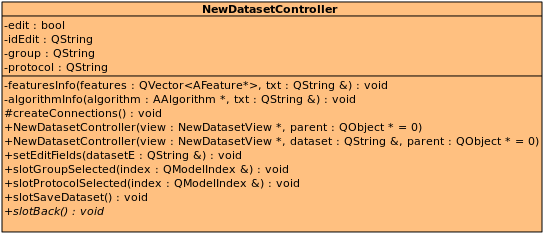
\includegraphics[width=0.7\linewidth]{./Content/Immagini/controller/NewDatasetController.png}
		\caption{Diagramma classe NewDatasetController}
	\end{figure}
	\paragraph{Descrizione:} classe che rappresenta un controller per un oggetto NewDatasetView e ha il compito di creare un nuovo Protocol\g{}.
	\paragraph{Utilizzo:} viene utilizzata per gestire i Signal\g{} emessi dall'oggetto NewDatasetView associato e reagisce in modo appropriato una volta recepito.
	\paragraph{Eredita da:}
		\begin{itemize}
			\item Romeo::Controller::AController.
		\end{itemize}
	\paragraph{Attributi}
		\begin{itemize}
			\item \color{teal} \verb!- edit : bool!
			\color{black}
			\subparagraph{Descrizione} rappresenta un flag che vale false se è un nuovo Dataset\g{} altrimenti vale true.
			\item \color{teal} \verb!- idEdit : QString!
			\color{black}
			\subparagraph{Descrizione} rappresenta l'id del Dataset\g{} da modificare.
			\item \color{teal} \verb!- group : QString!
			\color{black}
			\subparagraph{Descrizione} rappresenta il gruppo contenuto all'interno del Dataset\g{}.
			\item \color{teal} \verb!- protocol : QString!
			\color{black}
			\subparagraph{Descrizione} rappresenta il protocol selezionato contenuto all'interno del Dataset\g{}.
		\end{itemize}
	\paragraph{\color{black}Metodi}
		\begin{itemize}
			\item \color{blue} \verb!- featureInfo(features : QVector<AFeature*>, txt : QString &) : void!
			\color{black}
			\subparagraph{Descrizione:} metodo che imposta le informazioni legate alle Feature\g{} contenute nel Dataset\g{}.
			\color{black}
			\subparagraph{Argomenti}
			\begin{itemize}
				\item \color{RoyalPurple} \verb!features : QVector<AFeature*>!\\				
\color{black} rappresenta l'insieme delle Feature\g{} contenute nel Dataset\g{}.
				\item \color{RoyalPurple} \verb!txt : QString &!\\				
\color{black} rappresenta la stringa alla quale vengono aggiunte le informazioni relative alle Feature\g{} contenute nel Dataset\g{}
			\end{itemize}
			\subparagraph{Note}
			\begin{itemize}
				\item Il metodo deve essere marcato come costante.
			\end{itemize}
			\item \color{blue} \verb!- algorithmInfo(algorithm : AAlgorihm *, txt : QString &) : void!
			\color{black}
			\subparagraph{Descrizione:} metodo che imposta le informazioni legate all'algoritmo di cluster\g{}  del Protocol\g{} contenuto dentro al Dataset\g{}.
			\color{black}
			\subparagraph{Argomenti}
			\begin{itemize}
				\item \color{RoyalPurple} \verb!algorithm : AAlgorihm *!\\				
\color{black} rappresenta l'algoritmo contenuto nel Protocol\g{}.
				\item \color{RoyalPurple} \verb!txt : QString &!\\				
\color{black} rappresenta la stringa nella quale verranno inserite le informazioni dell'algoritmo di cluster\g{}.
			\end{itemize}
			\subparagraph{Note}
			\begin{itemize}
				\item Il metodo deve essere marcato come costante.
			\end{itemize}
			\item \color{blue} \verb!# createConnections() : void!
			\color{black}
			\subparagraph{Descrizione} metodo che crea le connessioni tra la vista associata all'oggetto controller in questione.
			\subparagraph{Note}
			\begin{itemize}
				\item Il metodo deve essere marcato come costante.
			\end{itemize}
			\item \color{blue} \verb!+ NewDatasetController(view : MainWindowController*, dataset : const QString &, parent : QObject *)!
			\color{black}
			\subparagraph{Descrizione:} costruttore per la classe NewDatasetController che riceve come parametro la view associata da gestire.
			\color{black}
			\subparagraph{Argomenti}
			\begin{itemize}
				\item \color{RoyalPurple} \verb!view : MainWindowController*!\\				
\color{black} rappresenta la view che verrà associata all'oggetto in creazione.
				\item \color{RoyalPurple} \verb!dataset : const QString &!\\				
\color{black} rappresenta il nome del Dataset\g{} da modificare.
				\item \color{RoyalPurple} \verb!parent : QObject *!\\				
\color{black} rappresenta il parent dell'oggetto in creazione.
			\end{itemize}
			\item \color{blue} \verb!+ NewDatasetController(view : NewDatasetView*, parent : QObject *)!
			\color{black}
			\subparagraph{Descrizione:} costruttore per la classe NewDatasetController al quale viene passata la view che gestirà, e il Dataset\g{} che l'utente vuole modificare.
			\color{black}
			\subparagraph{Argomenti}
			\begin{itemize}
				\item \color{RoyalPurple} \verb!view : NewDatasetView*!\\				
\color{black} rappresenta la view che verrà associata al controller in creazione.
				\item \color{RoyalPurple} \verb!parent : QObject *!\\				
\color{black} rappresenta il parent dell'oggetto in creazione.
			\end{itemize}
			\item \color{blue} \verb!+ setEditFields(datasetE : const QString &) : void!
			\color{black}
			\subparagraph{Descrizione:} metodo che imposta i campi dati per poter essere modificati dall'utente.
			\color{black}
			\subparagraph{Argomenti}
			\begin{itemize}
				\item \color{RoyalPurple} \verb!datasetE : const QString &!\\				
\color{black} rappresenta il nome del Dataset\g{} da modificare.
			\end{itemize}
			\item \color{blue} \verb!- slotGroupSelected(index : const QModelIndex &, index : const QModelIndex &) : void!
			\color{black}
			\subparagraph{Descrizione:} Slot\g{} che riceve il segnale della selezione, da parte dell'utente, del gruppo di Subject\g{}.
			\color{black}
			\subparagraph{Argomenti}
			\begin{itemize}
				\item \color{RoyalPurple} \verb!index : const QModelIndex &!\\				
\color{black} rappresenta l'indice della tabella cui si trova il gruppo di Subject\g{} selezionato.
				\item \color{RoyalPurple} \verb!index : const QModelIndex &!\\				
\color{black} rappresenta l'indice della tabella cui si trova il Protocol\g{} selezionato.
			\end{itemize}
			\subparagraph{Note}
			\begin{itemize}
				\item Il metodo è uno slot\g{} Qt\g{}.
			\end{itemize}
			\item \color{blue} \verb!+ slotProtocolSelected() : void!
			\color{black}
			\subparagraph{Descrizione} Slot\g{} che riceve il segnale della selezione, da parte dell'utente, del Protocol\g{}.
			\subparagraph{Note}
			\begin{itemize}
				\item Il metodo è uno slot\g{} Qt\g{}.
			\end{itemize}
			\item \color{blue} \verb!+ slotSaveDataset() : void!
			\color{black}
			\subparagraph{Descrizione} Slot\g{} che riceve il segnale della selezione, da parte dell'utente, del pulstante per il salvataggio delle modifiche (save).
			\subparagraph{Note}
			\begin{itemize}
				\item Il metodo è uno slot\g{} Qt\g{}.
			\end{itemize}
			\item \color{blue} \verb!+ slotBack() : void!
			\color{black}
			\subparagraph{Descrizione} Slot\g{}  virtuale che implementa il contratto di ritorno alla view precedente e reagisce al segnale della pressione del pulsante back dalla view. In particolare ritorna alla finestra principale se le modifiche fatte riguardano la creazione di un nuovo Dataset\g{} altrimenti ritorna alla view che mostra tutti i Dataset\g{} presenti all'interno del sistema.
			\subparagraph{Note}
			\begin{itemize}
				\item Il metodo deve essere marcato come virtuale.
				\item Il metodo è uno slot\g{} Qt\g{}.
			\end{itemize}
		\end{itemize}
		\pagebreak
	\subsubsection{NewGroupController (class)}
	\begin{figure}[!h]
		\centering
		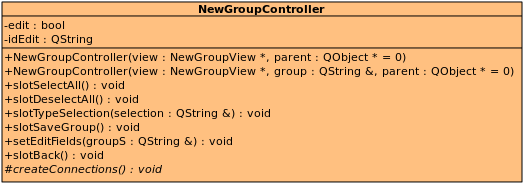
\includegraphics[width=0.7\linewidth]{./Content/Immagini/controller/NewGroupController}
		\caption{Diagramma classe \textsl{NewGroupController}}
	\end{figure}
	\paragraph{Descrizione:} classe rappresentante un controller per un oggetto di tipo \textsl{NewGroupView}.
	\paragraph{Utilizzo:} gestisce i signal\g{} emessi da un oggetto \textsl{NewGroupView} ed agisce conseguentemente in modo appropriato.
	\paragraph{Eredita da:}
		\begin{itemize}
			\item Romeo::Controller::AController.
		\end{itemize}
	\paragraph{Attributi}
		\begin{itemize}
			\item \color{teal} \verb!# edit : bool!
			\color{black}
			\subparagraph{Descrizione} Rappresenta il tipo di operazione svolta dal controller. Nel caso in cui valga \verb!true!, il controller si occuperà di gestire la modifica di un gruppo di \subject{}. In caso contrario, gestirà la creazione di un nuovo gruppo.
			\item \color{teal} \verb!- idEdit : QString!
			\color{black}
			\subparagraph{Descrizione} Stringa rappresentante il nome del gruppo di \subject{} che si vuole eventualmente modificare.
		\end{itemize}
	\paragraph{\color{black}Metodi}
		\begin{itemize}
			\item \color{blue} \verb!# createConnections() : void!
			\color{black}
			\subparagraph{Descrizione} Metodo che si occupa di creare le connessioni tra i segnali emessi dalla vista associata e gli slot\g{} dell'oggetto \textsl{NewGroupController}.
			\subparagraph{Note}
			\begin{itemize}
				\item Il metodo deve essere marcato come costante.
				\item Il metodo deve essere marcato come virtuale.
			\end{itemize}
			\item \color{blue} \verb!+ NewGroupController(view : NewGroupView *, parent : QObject *)!
			\color{black}
			\subparagraph{Descrizione:} Costruttore della classe \textsl{NewGroupController}. Si occupa di costruire un oggetto di tipo \textsl{NewGroupController}, associandolo alla propria vista. Tale costruttore viene utilizzato quando è necessario gestire una vista di creazione di un nuovo gruppo di \subject{}.
			\color{black}
			\subparagraph{Argomenti}
			\begin{itemize}
				\item \color{RoyalPurple} \verb!view : NewGroupView *!\\				
\color{black} Puntatore all'oggetto di tipo \textsl{NewGroupView}, rappresentante la vista che verrà controllata dall'oggetto \textsl{NewGroupController}.
				\item \color{RoyalPurple} \verb!parent : QObject *!\\				
\color{black} Puntatore all'oggetto \textsl{QObject}, rappresentante il padre dell'oggetto \textsl{NewGroupController}.
			\end{itemize}
			\item \color{blue} \verb!+ NewGroupController(view : NewGroupView *, group : const QString &,! \\ \verb! parent : QObject *)!
			\color{black}
			\subparagraph{Descrizione:} Costruttore della classe \textsl{NewGroupController}. Si occupa di costruire un oggetto di tipo \textsl{NewGroupController}, associandolo alla propria vista. Tale costruttore viene utilizzato quando è necessario gestire una modifica ad un gruppo di \subject{} preesistente.
			\color{black}
			\subparagraph{Argomenti}
			\begin{itemize}
				\item \color{RoyalPurple} \verb!view : NewGroupView *!\\				
\color{black} Puntatore all'oggetto di tipo \textsl{NewGroupView}, rappresentante la vista che verrà controllata dall'oggetto \textsl{NewGroupController}.
				\item \color{RoyalPurple} \verb!group : const QString &!\\				
\color{black} Stringa rappresentante il nome del gruppo di \subject{} di cui il controller deve gestire le modifiche.
				\item \color{RoyalPurple} \verb!parent : QObject *!\\				
\color{black} Puntatore all'oggetto \textsl{QObject}, rappresentante il padre dell'oggetto \textsl{NewGroupController}.
			\end{itemize}
			\item \color{blue} \verb!+ slotSelectAll() : void!
			\color{black}
			\subparagraph{Descrizione} Metodo che permette di selezionare tutti i \subject{} presenti nel sistema, per aggiungerli al gruppo di \subject{} che l'utente sta creando.
			\subparagraph{Note}
			\begin{itemize}
				\item Il metodo è uno slot\g{} Qt\g{}.
			\end{itemize}
			\item \color{blue} \verb!+ slotDeselectAll() : void!
			\color{black}
			\subparagraph{Descrizione} Metodo che permette di deselezionare tutti i \subject{} presenti nella view.
			\subparagraph{Note}
			\begin{itemize}
				\item Il metodo è uno slot\g{} Qt\g{}.
			\end{itemize}
			\item \color{blue} \verb!+ slotTypeSelection(selection : const QString &) : void!
			\color{black}
			\subparagraph{Descrizione:} Metodo che gestisce il cambiamento del tipo di gruppo che l'utente vuole creare (2D, 2D-t, 3D, 3D-t). Al cambiamento del tipo di gruppo da parte dell'utente, il controller si occupa di aggiornare i \subject{} presenti nel sistema, con quelli della tipologia selezionata.
			\color{black}
			\subparagraph{Argomenti}
			\begin{itemize}
				\item \color{RoyalPurple} \verb!selection : const QString &!\\				
\color{black} Stringa rappresentante il nuovo tipo di gruppo di \subject{} che l'utente vuole creare.
			\end{itemize}
			\subparagraph{Note}
			\begin{itemize}
				\item Il metodo è uno slot\g{} Qt\g{}.
			\end{itemize}
			\item \color{blue} \verb!+ slotSaveGroup() : void!
			\color{black}
			\subparagraph{Descrizione} Metodo che gestise il salvataggio del gruppo di \subject{} che l'utente sta creando. Nel caso in cui i dati inseriti dall'utente non siano corretti, o siano incompleti, il controller crea una vista per segnalare all'utente il problema.
			\subparagraph{Note}
			\begin{itemize}
				\item Il metodo è uno slot\g{} Qt\g{}.
			\end{itemize}
			\item \color{blue} \verb!+ setEditFields(groupS : const QString &) : void!
			\color{black}
			\subparagraph{Descrizione:} Metodo che permette di visualizzare i dati di un determinato gruppo di \subject{}, nella vista associata.
			\color{black}
			\subparagraph{Argomenti}
			\begin{itemize}
				\item \color{RoyalPurple} \verb!groupS : const QString &!\\				
\color{black} Stringa rappresentante il nome del gruppo di \subject{} di cui si vogliono visualizzare i dati nella rispettiva vista.
			\end{itemize}
			\subparagraph{Note}
			\begin{itemize}
				\item Il metodo è uno slot\g{} Qt\g{}.
			\end{itemize}
			\item \color{blue} \verb!+ slotBack() : void!
			\color{black}
			\subparagraph{Descrizione} Metodo che permette di ritornare alla vista precedentemente visualizzata. Tale vista cambierà in base alla tipologia di operazione che l'utente sta compiendo (modifica o creazione di un gruppo).
			\subparagraph{Note}
			\begin{itemize}
				\item Il metodo deve essere marcato come virtuale.
				\item Il metodo è uno slot\g{} Qt\g{}.
			\end{itemize}
			\item \color{blue} \verb!- create_Update(group : GroupOfSubject*, name : QString &) : void!
			\color{black}
			\subparagraph{Descrizione:} metodo che ha il compito di salvare o aggiornare un gruppo di Subject\g{} all'interno del database,
			\color{black}
			\subparagraph{Argomenti}
			\begin{itemize}
				\item \color{RoyalPurple} \verb!group : GroupOfSubject*!\\				
\color{black} puntatore al gruppo da salvare o aggiornare.
				\item \color{RoyalPurple} \verb!name : QString &!\\				
\color{black} riferimento al nome del gruppo passato come parametro.
			\end{itemize}
		\end{itemize}
		\pagebreak
	\subsubsection{NewProtocolController (class)}
	\begin{figure}[!h]
		\centering
		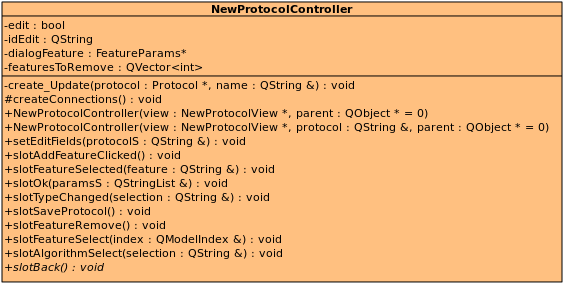
\includegraphics[width=0.75\linewidth]{./Content/Immagini/controller/NewProtocolController.png}
		\caption{Diagramma classe NewProtocolController}
	\end{figure}
	\paragraph{Descrizione:} classe che rappresenta un controller per un oggetto NewProtocolView e ha il compito di gestire un nuovo Protocol\g{}
	\paragraph{Utilizzo:} viene utilizzata per gestire i Signal\g{} emessi da un oggetto NewProtocolview e reagisce in modo appropriato ad essi una volta catturati
	\paragraph{Eredita da:}
		\begin{itemize}
			\item Romeo::Controller::AController.
		\end{itemize}
	\paragraph{Attributi}
		\begin{itemize}
			\item \color{teal} \verb!- edit : bool!
			\color{black}
			\subparagraph{Descrizione} rappresenta un flag che vale false se si sta creando un nuovo Protocol\g{}, true altrimenti.
			\item \color{teal} \verb!- idEdit : QString!
			\color{black}
			\subparagraph{Descrizione} rappresenta l'id del Protocol\g{} che l'utente sta modificando.
			\item \color{teal} \verb!- dialogFeature : FeatureParams*!
			\color{black}
			\subparagraph{Descrizione} rappresenta la finestra di dialogo adibita all'aggiunta di una Feature\g{}.
			\item \color{teal} \verb!- featuresToRemove : QVector<int>!
			\color{black}
			\subparagraph{Descrizione} rappresenta l'insieme di id delle Feature\g{} che l'utente vuole rimuovere dal Protocol\g{}.
		\end{itemize}
	\paragraph{\color{black}Metodi}
		\begin{itemize}
			\item \color{blue} \verb!- create_Update(protocol : Protocol*, parent : QObject *) : void!
			\color{black}
			\subparagraph{Descrizione:} metodo che ha il compito di salvare o aggiornare il Protocol\g{} in questione.
			\color{black}
			\subparagraph{Argomenti}
			\begin{itemize}
				\item \color{RoyalPurple} \verb!protocol : Protocol*!\\				
\color{black} rappresenta il Protocol\g{} da salvare o modificare a seconda che il Protocol\g{} sia in creazione o precedentemente creato e ora in modifica.
				\item \color{RoyalPurple} \verb!parent : QObject *!\\				
\color{black} rappresenta il parent  dell'oggetto in creazione.
			\end{itemize}
			\item \color{blue} \verb!# createConnections() : void!
			\color{black}
			\subparagraph{Descrizione} metodo che ha il compito di creare tutte le connessioni tra l'oggetto controller e la view associata ad esso da gestire.
			\subparagraph{Note}
			\begin{itemize}
				\item Il metodo deve essere marcato come costante.
			\end{itemize}
			\item \color{blue} \verb!+ NewProtocolController(view : NewProtocolView*, parent : QObject *)!
			\color{black}
			\subparagraph{Descrizione:} costruttore per un oggetto NewProtocolController a cui viene passata la view gestita dall'oggetto che si sta creando.
			\color{black}
			\subparagraph{Argomenti}
			\begin{itemize}
				\item \color{RoyalPurple} \verb!view : NewProtocolView*!\\				
\color{black} rappresenta la view che verrà associata all'oggetto controller in creazione.
				\item \color{RoyalPurple} \verb!parent : QObject *!\\				
\color{black} rappresenta il parent dell'oggetto in creazione.
			\end{itemize}
			\item \color{blue} \verb!+ NewProtocolController(view : NewProtocolView*, protocol : const QString &, parent : QObject *)!
			\color{black}
			\subparagraph{Descrizione:} costruttore per l'oggetto controller che gestisce la view NewProtocolView quando l'utente vuole modificare il Protocol\g{} precedentemente selezionato.
			\color{black}
			\subparagraph{Argomenti}
			\begin{itemize}
				\item \color{RoyalPurple} \verb!view : NewProtocolView*!\\				
\color{black} rappresenta la view che verrà associata all'oggetto controller in creazione.
				\item \color{RoyalPurple} \verb!protocol : const QString &!\\				
\color{black} stringa che rappresenta il nome del Protocol\g{} che l'utente ha scelto di modificare
				\item \color{RoyalPurple} \verb!parent : QObject *!\\				
\color{black} rappresenta il parent del controller in creazione.
			\end{itemize}
			\item \color{blue} \verb!+ setEditFields(protocolS : const QString &) : void!
			\color{black}
			\subparagraph{Descrizione:} metodo che ha il compito di impostare i campi in modo tale che l'utente possa modificarne i valori.
			\color{black}
			\subparagraph{Argomenti}
			\begin{itemize}
				\item \color{RoyalPurple} \verb!protocolS : const QString &!\\				
\color{black} la stringa rappresenta il nome del Protocol\g{} i cui campi devono essere preparati per la possibile modifica da parte dell'utente.
			\end{itemize}
			\item \color{blue} \verb!+ slotAddFeatureClicked() : void!
			\color{black}
			\subparagraph{Descrizione} Slot\g{} che ha il compito di aggiungere la Feature\g{} selezionata dalla finestra di dialogo contenente le Feature\g{} disponibili.
			\subparagraph{Note}
			\begin{itemize}
				\item Il metodo è uno slot\g{} Qt\g{}.
			\end{itemize}
			\item \color{blue} \verb!+ slotFeatureSelected(feature : const QString &) : void!
			\color{black}
			\subparagraph{Descrizione:} Slot\g{} che riceve il segnale quando l'utente seleziona una Feature\g{} dalla finestra di dialogo per l'inserimento di una nuova Feature\g{}
			\color{black}
			\subparagraph{Argomenti}
			\begin{itemize}
				\item \color{RoyalPurple} \verb!feature : const QString &!\\				
\color{black} rappresenta il nome della Feature\g{} selezionata.
			\end{itemize}
			\subparagraph{Note}
			\begin{itemize}
				\item Il metodo è uno slot\g{} Qt\g{}.
			\end{itemize}
			\item \color{blue} \verb!+ slotOk(paramsS : const QStringList&) : void!
			\color{black}
			\subparagraph{Descrizione:} Slot\g{} che ha il compito di aggiungere al Protocol\g{} la Feature\g{} aggiunta dall'utente.
			\color{black}
			\subparagraph{Argomenti}
			\begin{itemize}
				\item \color{RoyalPurple} \verb!paramsS : const QStringList&!\\				
\color{black} rappresenta la lista dei valori dei parametri della Feature\g{} da aggiungere al Protocol\g{} in creazione.
			\end{itemize}
			\subparagraph{Note}
			\begin{itemize}
				\item Il metodo è uno slot\g{} Qt\g{}.
			\end{itemize}
			\item \color{blue} \verb!+ slotTypeChanged(selection : const QString &) : void!
			\color{black}
			\subparagraph{Descrizione:} Slot\g{} che ha il compito di modificare il tipo associato al Protocol\g{} che l'utente vuole andare  a creare. Lo Slot\g{} aggiorna la view associata che ha lanciato il Signal\g{} con le informazioni appropriate.
			\color{black}
			\subparagraph{Argomenti}
			\begin{itemize}
				\item \color{RoyalPurple} \verb!selection : const QString &!\\				
\color{black} rappresenta il tipo, che l'utente ha selezionato, associato al Protocol\g{} in creazione.
			\end{itemize}
			\subparagraph{Note}
			\begin{itemize}
				\item Il metodo è uno slot\g{} Qt\g{}.
			\end{itemize}
			\item \color{blue} \verb!+ slotSaveProtocol() : void!
			\color{black}
			\subparagraph{Descrizione} Slot\g{} che ha il compito di salvare il Protocol\g{} nell'applicativo Romeo una volta che l'utente preme sul pulsante save della view associata al controller che riceve il Signal\g{}.
			\subparagraph{Note}
			\begin{itemize}
				\item Il metodo è uno slot\g{} Qt\g{}.
			\end{itemize}
			\item \color{blue} \verb!+ slotFeatureRemove() : void!
			\color{black}
			\subparagraph{Descrizione} Slot\g{} che ha il compito di rimuovere dal Protocol\g{} le Feature\g{} selezionate dall'utente nella view associata al controller che riceve il Signal\g{}.
			\subparagraph{Note}
			\begin{itemize}
				\item Il metodo è uno slot\g{} Qt\g{}.
			\end{itemize}
			\item \color{blue} \verb!+ slotFeatureSelect(index : const QModelIndex &) : void!
			\color{black}
			\subparagraph{Descrizione:} Slot\g{} che riceve il segnale dalla view associata quando l'utente seleziona una Feature\g{} dalla tabella contenente tutte le Feature\g{} presenti nell'applicativo Romeo.
			\color{black}
			\subparagraph{Argomenti}
			\begin{itemize}
				\item \color{RoyalPurple} \verb!index : const QModelIndex &!\\				
\color{black} rappresenta l'indice della tabella che è stato selezionato.
			\end{itemize}
			\subparagraph{Note}
			\begin{itemize}
				\item Il metodo è uno slot\g{} Qt\g{}.
			\end{itemize}
			\item \color{blue} \verb!+ slotAlgorithm(selection : const QString &) : void!
			\color{black}
			\subparagraph{Descrizione:} Slot\g{} che riceve il segnale dalla view associata quando l'utente seleziona l'algoritmo di cluster\g{}.
			\color{black}
			\subparagraph{Argomenti}
			\begin{itemize}
				\item \color{RoyalPurple} \verb!selection : const QString &!\\				
\color{black} rappresenta il nome dell'algortimo di cluster\g{} che l'utente ha selezionato.
			\end{itemize}
			\subparagraph{Note}
			\begin{itemize}
				\item Il metodo è uno slot\g{} Qt\g{}.
			\end{itemize}
			\item \color{blue} \verb!+ slotBack() : void!
			\color{black}
			\subparagraph{Descrizione} Slot\g{}  virtuale che ha il compito di ritornare alla precedente view visualizzata dall'utente.
			\subparagraph{Note}
			\begin{itemize}
				\item Il metodo deve essere marcato come virtuale.
				\item Il metodo è uno slot\g{} Qt\g{}.
			\end{itemize}
		\end{itemize}
		\pagebreak
	\subsubsection{NewSubjectController (class)}
	\begin{figure}[!h]
		\centering
		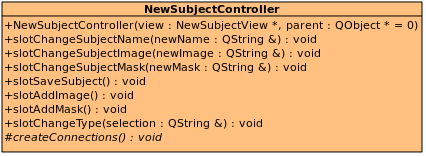
\includegraphics[width=0.7\linewidth]{./Content/Immagini/controller/NewSubjectController.png}
		\caption{Diagramma classe \textsl{NewSubjectController}}
	\end{figure}
	\paragraph{Descrizione:} classe rappresentante un controller per un oggetto di tipo \textsl{NewSubjectView}.
	\paragraph{Utilizzo:} gestisce i signal\g{} emessi da un oggetto \textsl{NewSubjectView} ed agisce conseguentemente in modo appropriato.
	\paragraph{Eredita da:}
		\begin{itemize}
			\item Romeo::Controller::AController.
		\end{itemize}
	\paragraph{\color{black}Metodi}
		\begin{itemize}
			\item \color{blue} \verb!# createConnections() : void!
			\color{black}
			\subparagraph{Descrizione} Metodo che si occupa di creare le connessioni tra i segnali emessi dalla vista associata e gli slot\g{} dell'oggetto \textsl{NewSubjectController}.
			\subparagraph{Note}
			\begin{itemize}
				\item Il metodo deve essere marcato come costante.
				\item Il metodo deve essere marcato come virtuale.
			\end{itemize}
			\item \color{blue} \verb!+ NewSubjectController(view : NewSubjectView *, parent : QObject *)!
			\color{black}
			\subparagraph{Descrizione:} Costruttore pubblico della classe \textsl{NewSubjectController}. Si occupa di costruire un oggetto di tipo \textsl{NewSubjectController}, associandolo alla propria vista.
			\color{black}
			\subparagraph{Argomenti}
			\begin{itemize}
				\item \color{RoyalPurple} \verb!view : NewSubjectView *!\\				
\color{black} Puntatore all'oggetto di tipo \textsl{NewSubjectView}, rappresentante la vista che verrà controllata dall'oggetto \textsl{NewSubjectController}.
				\item \color{RoyalPurple} \verb!parent : QObject *!\\				
\color{black} Puntatore all'oggetto \textsl{QObject}, rappresentante il padre dell'oggetto \textsl{NewSubjectController}.
			\end{itemize}
			\item \color{blue} \verb!+ slotChangeSubjectName(newName : const QString &) : void!
			\color{black}
			\subparagraph{Descrizione:} Metodo che gestisce il cambiamento di nome del \subject{} che l'utente sta creando.
			\color{black}
			\subparagraph{Argomenti}
			\begin{itemize}
				\item \color{RoyalPurple} \verb!newName : const QString &!\\				
\color{black} Stringa rappresentante il nuovo nome che l'utente vuole assegnare al \subject{}.
			\end{itemize}
			\subparagraph{Note}
			\begin{itemize}
				\item Il metodo è uno slot\g{} Qt\g{}.
			\end{itemize}
			\item \color{blue} \verb!+ slotChangeSubjectImage(newImage : const QString &) : void!
			\color{black}
			\subparagraph{Descrizione:} Metodo che gestisce il cambiamento dell'immagine del \subject{} che l'utente sta creando.
			\color{black}
			\subparagraph{Argomenti}
			\begin{itemize}
				\item \color{RoyalPurple} \verb!newImage : const QString &!\\				
\color{black} Stringa rappresentante la nuova immagine che l'utente vuole assegnare al \subject{}.
			\end{itemize}
			\subparagraph{Note}
			\begin{itemize}
				\item Il metodo è uno slot\g{} Qt\g{}.
			\end{itemize}
			\item \color{blue} \verb!+ slotChangeSubjectMask(newMask : const QString &) : void!
			\color{black}
			\subparagraph{Descrizione:} Metodo che gestisce il cambiamento della maschera del \subject{} che l'utente sta creando.
			\color{black}
			\subparagraph{Argomenti}
			\begin{itemize}
				\item \color{RoyalPurple} \verb!newMask : const QString &!\\				
\color{black} Stringa rappresentante la nuova maschera che l'utente vuole assegnare al \subject{}.
			\end{itemize}
			\subparagraph{Note}
			\begin{itemize}
				\item Il metodo è uno slot\g{} Qt\g{}.
			\end{itemize}
			\item \color{blue} \verb!+ slotSaveSubject() : void!
			\color{black}
			\subparagraph{Descrizione} Metodo che si occupa di salvare nel database il \subject{} che l'utente sta creando.
			\subparagraph{Note}
			\begin{itemize}
				\item Il metodo è uno slot\g{} Qt\g{}.
			\end{itemize}
			\item \color{blue} \verb!+ slotAddImage() : void!
			\color{black}
			\subparagraph{Descrizione} Metodo che crea la finestra di dialogo che permette all'utente di selezionare dal filesystem, il file contenente l'immagine da associare al \subject{} che l'utente sta creando.
			\subparagraph{Note}
			\begin{itemize}
				\item Il metodo è uno slot\g{} Qt\g{}.
			\end{itemize}
			\item \color{blue} \verb!+ slotAddMask() : void!
			\color{black}
			\subparagraph{Descrizione} Metodo che crea la finestra di dialogo che permette all'utente di selezionare dal filesystem, il file contenente la maschera da associare al \subject{} che l'utente sta creando.
			\subparagraph{Note}
			\begin{itemize}
				\item Il metodo è uno slot\g{} Qt\g{}.
			\end{itemize}
			\item \color{blue} \verb!+ slotChangeType(selection : const QString &) : void!
			\color{black}
			\subparagraph{Descrizione:} Metodo che gestisce il cambiamento del tipo di \subject{} che l'utente sta creando.
			\color{black}
			\subparagraph{Argomenti}
			\begin{itemize}
				\item \color{RoyalPurple} \verb!selection : const QString &!\\				
\color{black} Stringa rappresentante il nuovo tipo che l'utente vuole assegnare al \subject{}.
			\end{itemize}
			\subparagraph{Note}
			\begin{itemize}
				\item Il metodo è uno slot\g{} Qt\g{}.
			\end{itemize}
			\item \color{blue} \verb!- creationDone(name : QString &, imagePath : QFileInfo&, image : QString &, mask : QString &, maskPath : QFileInfo&) : void!
			\color{black}
			\subparagraph{Descrizione:} metodo che ha il compito di copiare il file caricato alla creazione del Subject\g{} da parte dell'utente e visualizza il messaggio di salvataggio.
			\color{black}
			\subparagraph{Argomenti}
			\begin{itemize}
				\item \color{RoyalPurple} \verb!name : QString &!\\				
\color{black} rappresenta il nome del Subject\g{} creato.
				\item \color{RoyalPurple} \verb!imagePath : QFileInfo&!\\				
\color{black} rappresenta il path a cui reperire l'immagine selezionata dall'utente\g{}.
				\item \color{RoyalPurple} \verb!image : QString &!\\				
\color{black} rappresenta il nome dell'immagine selezionata dall'utente.
				\item \color{RoyalPurple} \verb!mask : QString &!\\				
\color{black} rappresenta il nome della maschera selezionata dall'utente.
				\item \color{RoyalPurple} \verb!maskPath : QFileInfo&!\\				
\color{black} rappresenta il path a cui reperire la maschera selezionata dall'utente.
			\end{itemize}
		\end{itemize}
		\pagebreak
	\subsubsection{ProtocolsController (class)}
	\begin{figure}[!h]
		\centering
		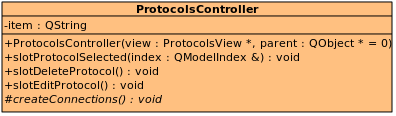
\includegraphics[width=0.6\linewidth]{./Content/Immagini/controller/ProtocolsController}
		\caption{Diagramma classe \textsl{ProtocolsController}}
	\end{figure}
	\paragraph{Descrizione:} classe rappresentante un controller per un oggetto di tipo \textsl{ProtocolsView}.
	\paragraph{Utilizzo:} gestisce i signal\g{} emessi da un oggetto \textsl{ProtocolsView} ed agisce conseguentemente in modo appropriato.
	\paragraph{Eredita da:}
		\begin{itemize}
			\item Romeo::Controller::AController.
		\end{itemize}
	\paragraph{Attributi}
		\begin{itemize}
			\item \color{teal} \verb!- item : QString!
			\color{black}
			\subparagraph{Descrizione} Rappresenta il nome del \protocol{} selezionato dall'utente nella vista associata al controller.
		\end{itemize}
	\paragraph{\color{black}Metodi}
		\begin{itemize}
			\item \color{blue} \verb!# createConnections() : void!
			\color{black}
			\subparagraph{Descrizione} Metodo che si occupa di creare le connessioni tra i segnali emessi dalla vista associata e gli slot\g{} dell'oggetto \textsl{ProtocolsController}.
			\subparagraph{Note}
			\begin{itemize}
				\item Il metodo deve essere marcato come costante.
				\item Il metodo deve essere marcato come virtuale.
			\end{itemize}
			\item \color{blue} \verb!+ ProtocolsController(view : ProtocolsView *, parent : QObject *)!
			\color{black}
			\subparagraph{Descrizione:} Costruttore pubblico della classe \textsl{ProtocolsController}. Si occupa di costruire un oggetto di tipo \textsl{ProtocolsController}, associandolo alla propria vista.
			\color{black}
			\subparagraph{Argomenti}
			\begin{itemize}
				\item \color{RoyalPurple} \verb!view : ProtocolsView *!\\				
\color{black} Puntatore all'oggetto di tipo \textsl{ProtocolsView}, rappresentante la vista che verrà controllata dall'oggetto \textsl{ProtocolsController}.
				\item \color{RoyalPurple} \verb!parent : QObject *!\\				
\color{black} Puntatore all'oggetto \textsl{QObject}, rappresentante il padre dell'oggetto \textsl{ProtocolsController}.
			\end{itemize}
			\item \color{blue} \verb!+ slotProtocolSelected(index : const QModelIndex &) : void!
			\color{black}
			\subparagraph{Descrizione:} Metodo che, successivamente alla richiesta dell'utente, imposta la vista con i dati del \protocol{} selezionato.
			\color{black}
			\subparagraph{Argomenti}
			\begin{itemize}
				\item \color{RoyalPurple} \verb!index : const QModelIndex &!\\				
\color{black} Indice dell'item associato al \protocol{} selezionato dall'utente.
			\end{itemize}
			\subparagraph{Note}
			\begin{itemize}
				\item Il metodo è uno slot\g{} Qt\g{}.
			\end{itemize}
			\item \color{blue} \verb!+ slotDeleteProtocol() : void!
			\color{black}
			\subparagraph{Descrizione} Metodo che si occupa di gestire l'eliminazione del \protocol{} selezionato dall'utente.
			\subparagraph{Note}
			\begin{itemize}
				\item Il metodo è uno slot\g{} Qt\g{}.
			\end{itemize}
			\item \color{blue} \verb!+ slotEditProtocol() : void!
			\color{black}
			\subparagraph{Descrizione} Metodo che permette all'utente di poter modificare il \protocol{} selezionato.
			\subparagraph{Note}
			\begin{itemize}
				\item Il metodo è uno slot\g{} Qt\g{}.
			\end{itemize}
			\item \color{blue} \verb!- featuresInfo(feats : QVector<AFeature*>) : void!
			\color{black}
			\subparagraph{Descrizione:} metodo che ha il compito di caricare le informazioni relative alle Feature\g{} contenute nel Protocol\g{} selezionato.
			\color{black}
			\subparagraph{Argomenti}
			\begin{itemize}
				\item \color{RoyalPurple} \verb!feats : QVector<AFeature*>!\\				
\color{black} rappresenta l'insieme delle Feature\g{}  contenute nel Protocol\g{} associato al controller in esame.
			\end{itemize}
			\subparagraph{Note}
			\begin{itemize}
				\item Il metodo deve essere marcato come costante.
			\end{itemize}
			\item \color{blue} \verb!- algorithmInfo(algorithm : AAlgorihm *) : void!
			\color{black}
			\subparagraph{Descrizione:} metodo che carica le informazioni relative all'algoritmo di cluster\g{} contenuto dentro al Protocol\g{} selezionato.
			\color{black}
			\subparagraph{Argomenti}
			\begin{itemize}
				\item \color{RoyalPurple} \verb!algorithm : AAlgorihm *!\\				
\color{black} rappresenta l'algoritmo contenuto dentro al Protocol\g{} selezionato.
			\end{itemize}
			\subparagraph{Note}
			\begin{itemize}
				\item Il metodo deve essere marcato come costante.
			\end{itemize}
		\end{itemize}
		\pagebreak
	\subsubsection{ResultsController (class)}
	\begin{figure}[!h]
		\centering
		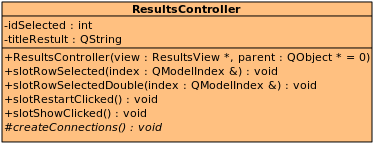
\includegraphics[width=0.6\linewidth]{./Content/Immagini/controller/ResultsController.png}
		\caption{Diagramma classe ResultsController}
	\end{figure}
	\paragraph{Descrizione:} classe che rappresenta un controller per un oggetto ResultsView.
	\paragraph{Utilizzo:} viene utilizzata per gestire i Signal\g{} emessi da un oggetto ResultsView e reagisce in modo appropriato a quelli recepiti.
	\paragraph{Eredita da:}
		\begin{itemize}
			\item Romeo::Controller::AController.
		\end{itemize}
	\paragraph{Attributi}
		\begin{itemize}
			\item \color{teal} \verb!- idSelected : int!
			\color{black}
			\subparagraph{Descrizione} rappresenta l'id dell'analisi selezionata all'interno del database.
			\item \color{teal} \verb!- titleResult : QString!
			\color{black}
			\subparagraph{Descrizione} rappresenta il titolo da visualizzare nella parte alta della view.
		\end{itemize}
	\paragraph{\color{black}Metodi}
		\begin{itemize}
			\item \color{blue} \verb!# createConnections() : void!
			\color{black}
			\subparagraph{Descrizione} metodo virtuale ridefinito che ha il compito di creare tutte le connessioni.
			\subparagraph{Note}
			\begin{itemize}
				\item Il metodo deve essere marcato come costante.
				\item Il metodo deve essere marcato come virtuale.
			\end{itemize}
			\item \color{blue} \verb!+ ResultsController(view : ResultsView*, parent : QObject *)!
			\color{black}
			\subparagraph{Descrizione:} Costruttore per la classe che associa l'oggetto in creazione con la view passata come parametro.
			\color{black}
			\subparagraph{Argomenti}
			\begin{itemize}
				\item \color{RoyalPurple} \verb!view : ResultsView*!\\				
\color{black} rappresenta la view a cui il controller in creazione verrà associata.
				\item \color{RoyalPurple} \verb!parent : QObject *!\\				
\color{black} rappresenta il parent del oggetto in creazione.
			\end{itemize}
			\item \color{blue} \verb!- slotRowSelected(index : const QModelIndex &) : void!
			\color{black}
			\subparagraph{Descrizione:} Slot\g{} che riceve il segnale dalla view associata quando l'utente seleziona la riga relativa a un'analisi.
			\color{black}
			\subparagraph{Argomenti}
			\begin{itemize}
				\item \color{RoyalPurple} \verb!index : const QModelIndex &!\\				
\color{black} rappresenta l'indice di riga della tabella selezionata.
			\end{itemize}
			\subparagraph{Note}
			\begin{itemize}
				\item Il metodo è uno slot\g{} Qt\g{}.
			\end{itemize}
			\item \color{blue} \verb!+ slotRowSelectedDouble(index : const QModelIndex &) : void!
			\color{black}
			\subparagraph{Descrizione:} Slot\g{} che riceve il segnale dalla view associata quando l'utente seleziona con il doppio click la riga relativa a un'analisi.
			\color{black}
			\subparagraph{Argomenti}
			\begin{itemize}
				\item \color{RoyalPurple} \verb!index : const QModelIndex &!\\				
\color{black} rappresenta l'indice di riga della tabella selezionata.
			\end{itemize}
			\subparagraph{Note}
			\begin{itemize}
				\item Il metodo è uno slot\g{} Qt\g{}.
			\end{itemize}
			\item \color{blue} \verb!+ slotRestarClicked() : void!
			\color{black}
			\subparagraph{Descrizione} Slot\g{} che riceve il segnale dalla view associata quando l'utente preme il pulsante di restart.
			\subparagraph{Note}
			\begin{itemize}
				\item Il metodo è uno slot\g{} Qt\g{}.
			\end{itemize}
			\item \color{blue} \verb!+ slotShowClicked() : void!
			\color{black}
			\subparagraph{Descrizione} Slot\g{} che riceve il segnale dalla view associata quando l'utente seleziona il pulsante per visualizzare i risultati dell'analisi.
			\subparagraph{Note}
			\begin{itemize}
				\item Il metodo è uno slot\g{} Qt\g{}.
			\end{itemize}
		\end{itemize}
		\pagebreak
	\subsubsection{SubjectsController (class)}
	\begin{figure}[!h]
		\centering
		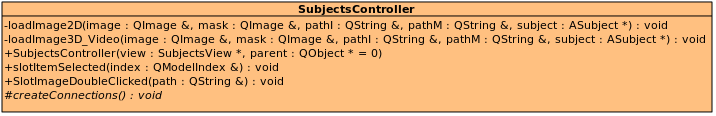
\includegraphics[width=\linewidth]{./Content/Immagini/controller/SubjectsController.png}
		\caption{Diagramma classe SubjectsController}
	\end{figure}
	\paragraph{Descrizione:} classe che rappresenta il controller per un oggetto SubjectView.
	\paragraph{Utilizzo:} Viene utilizzata per gesitre i Signal\g{} emessi da un oggetto SubjectsView e reagisce in modo appropriato ogni volta che ne cattura uno.
	\paragraph{Eredita da:}
		\begin{itemize}
			\item Romeo::Controller::AController.
		\end{itemize}
	\paragraph{\color{black}Metodi}
		\begin{itemize}
			\item \color{blue} \verb!- loadImage2D(image : QImage&, mask : QImage&, pathI : QString &, pathM : QString &, subject : ASubject*) : void!
			\color{black}
			\subparagraph{Descrizione:} metodo che carica un'immagine 2D associata al Subject\g{}
			\color{black}
			\subparagraph{Argomenti}
			\begin{itemize}
				\item \color{RoyalPurple} \verb!image : QImage&!\\				
\color{black} rappresenta l'immagine da caricare
				\item \color{RoyalPurple} \verb!mask : QImage&!\\				
\color{black} rappresenta la maschera da caricare
				\item \color{RoyalPurple} \verb!pathI : QString &!\\				
\color{black} rappresenta il path relativo all'immagine all'interno del filesystem.
				\item \color{RoyalPurple} \verb!pathM : QString &!\\				
\color{black} rappresenta il path relativo alla maschera all'interno del filesystem.
				\item \color{RoyalPurple} \verb!subject : ASubject*!\\				
\color{black} rappresenta il puntatore al Subject\g{} a cui sono associati immagine e maschera.
			\end{itemize}
			\item \color{blue} \verb!- loadImage3D_Video(image : QImage&, mask : QImage&, pathI : QString &,! \\ \verb! pathM : QString &, subject : ASubject*) : void!
			\color{black}
			\subparagraph{Descrizione:} metodo che carica un'immagine 3D o un video 2D/3D associata al Subject{}.
			\color{black}
			\subparagraph{Argomenti}
			\begin{itemize}
				\item \color{RoyalPurple} \verb!image : QImage&!\\				
\color{black} rappresenta l'immagine 3D o il video 2D/3D  da caricare.
				\item \color{RoyalPurple} \verb!mask : QImage&!\\				
\color{black} rappresenta la maschera da caricare.
				\item \color{RoyalPurple} \verb!pathI : QString &!\\				
\color{black} rappresenta il path relativo al file da caricare all'interno del filesystem
				\item \color{RoyalPurple} \verb!pathM : QString &!\\				
\color{black} rappresenta il path relativo alla maschera all'interno del filesystem.
				\item \color{RoyalPurple} \verb!subject : ASubject*!\\				
\color{black} rappresenta il Subject\g{} a cui associare i file passati come parametri ai metodi.
			\end{itemize}
			\item \color{blue} \verb!+ SubjectsController(view : SubjectView*, parent : QObject *)!
			\color{black}
			\subparagraph{Descrizione:} costruttore che ha il compito di costruire il controller associato alla view passata come parametro.
			\color{black}
			\subparagraph{Argomenti}
			\begin{itemize}
				\item \color{RoyalPurple} \verb!view : SubjectView*!\\				
\color{black} rappresenta il puntatore alla view cui il controller in costruzione verrà associato.
				\item \color{RoyalPurple} \verb!parent : QObject *!\\				
\color{black} rappresenta il parent di SubjectsController.
			\end{itemize}
			\item \color{blue} \verb!# createConnections() : void!
			\color{black}
			\subparagraph{Descrizione} metodo che ha il compito di creare tutte le connessioni per il controller.
			\subparagraph{Note}
			\begin{itemize}
				\item Il metodo deve essere marcato come virtuale.
				\item Il metodo deve essere marcato const.
			\end{itemize}
			\item \color{blue} \verb!+ slotItemSelected(item : const QModelIndex &) : void!
			\color{black}
			\subparagraph{Descrizione:} slot\g{} che mostra all'utente i dettagli del Subject\g{} selezionato nella view a cui il controller è associato.
			\color{black}
			\subparagraph{Argomenti}
			\begin{itemize}
				\item \color{RoyalPurple} \verb!item : const QModelIndex &!\\				
\color{black} rappresenta l'indice dell'elemento associato al Subject\g{} selezionato
			\end{itemize}
			\subparagraph{Note}
			\begin{itemize}
				\item Il metodo è uno slot\g{} Qt\g{}.
			\end{itemize}
			\item \color{blue} \verb!+ slotImageClicked(path : QString) : void!
			\color{black}
			\subparagraph{Descrizione:} Slot\g{} che riceve il Signal\g{} di doppio click dell'utente sull'anteprima dell'immagine o del video.
			\color{black}
			\subparagraph{Argomenti}
			\begin{itemize}
				\item \color{RoyalPurple} \verb!path : QString!\\				
\color{black} rappresenta il path del file selezionato
			\end{itemize}
			\subparagraph{Note}
			\begin{itemize}
				\item Il metodo è uno slot\g{} Qt\g{}.
			\end{itemize}
		\end{itemize}
		\pagebreak
	\subsubsection{WelcomeController (class)}
	\begin{figure}[!h]
		\centering
		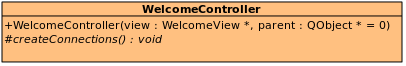
\includegraphics[width=0.6\linewidth]{./Content/Immagini/controller/WelcomeController}
		\caption{Diagramma classe \textsl{WelcomeController}}
	\end{figure}
	\paragraph{Descrizione:} classe che rappresenta un controller per un oggetto di tipo \textsl{WelcomeView}.
	\paragraph{Utilizzo:} gestisce i signal\g{} emessi da un oggetto \textsl{WelcomeView} ed agisce conseguentemente in modo appropriato.
	\paragraph{Eredita da:}
		\begin{itemize}
			\item Romeo::Controller::AController.
		\end{itemize}
	\paragraph{\color{black}Metodi}
		\begin{itemize}
			\item \color{blue} \verb!+ WelcomeController(view : WelcomeView *, parent : QObject *)!
			\color{black}
			\subparagraph{Descrizione:} Costruttore protetto della classe \textsl{WelcomeController}. Si occupa di costruire un oggetto di tipo \textsl{WelcomeController}, associandolo alla propria vista.
			\color{black}
			\subparagraph{Argomenti}
			\begin{itemize}
				\item \color{RoyalPurple} \verb!view : WelcomeView *!\\				
\color{black} Puntatore all'oggetto di tipo \textsl{WelcomeView}, rappresentante la vista che verrà controllata dall'oggetto \textsl{WelcomeController}.
				\item \color{RoyalPurple} \verb!parent : QObject *!\\				
\color{black} Puntatore all'oggetto \textsl{QObject}, rappresentante il padre dell'oggetto \textsl{WelcomeController}.
			\end{itemize}
			\item \color{blue} \verb!# createConnections() : void!
			\color{black}
			\subparagraph{Descrizione} Metodo che si occupa di creare le connessioni tra i segnali emessi dalla vista associata e gli slot\g{} dell'oggetto \textsl{WelcomeController}. Per l'implementazione del metodo, la classe utilizza gli slot forniti dalla classe \textsl{MainWindowController}.
			\subparagraph{Note}
			\begin{itemize}
				\item Il metodo deve essere marcato come costante.
				\item Il metodo deve essere marcato come virtuale.
			\end{itemize}
		\end{itemize}\begin{flushleft}
\end{flushleft}